\subsection{Briefing avec Leon Turrou}

\paragraph{} Pour les investigateurs, le scénario commence par une rencontre avec \gls{lgt}, dans le bureau qu'il occupe dans 
un commissariat de New York City. Sommairement, l'agent les informe que le Bureau vient de les réaffecter en renfort à sa
\emph{task force} sur le \emph{Lindberg Case}. Leur arrivée est appréciable, car il y a beaucoup à faire, mais le dossier 
est vaste, il va être difficile de vite les mettre à niveau. ``En conséquence, le Directeur et moi avons commencé par confier
un tâche ne nécessitant pas une connaissance profonde du dossier : l'arrestation de \gls{gms} !''.

\begin{wrapfigure}{r}{50mm}
\begin{center}
 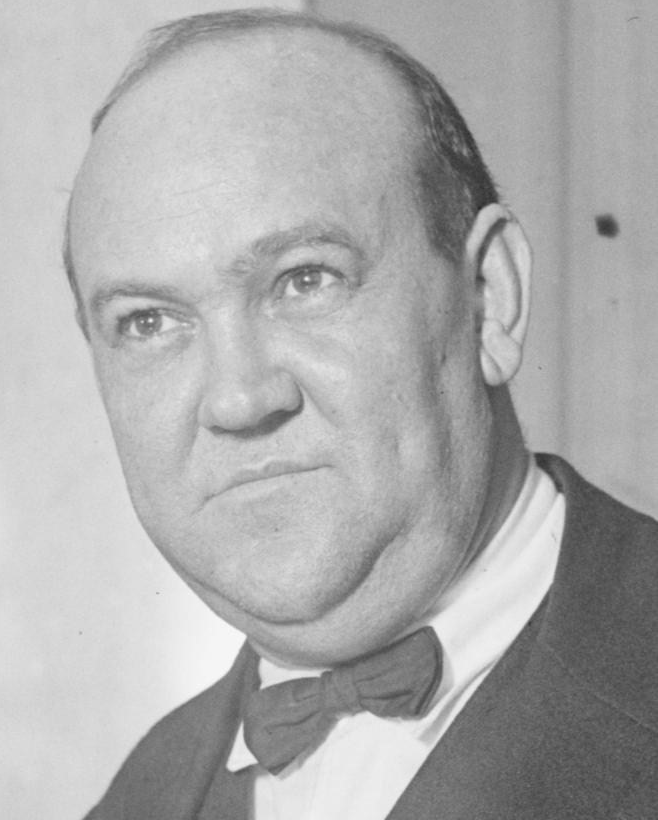
\includegraphics[width=40mm]{../pnjs/gaston-means-1924.png}
\end{center}
\caption{Gaston Means - 1924}
\end{wrapfigure}

\paragraph{} \gls{lgt} rappel sommairement le ``brillant'' parcours de \gls{gms} au sein du \gls{fbi} et décris sommairement
comment il a profité de l'affaire Lindbergh pour escroquer la jeune héritière. Il ajoute qu'il est fort content que cet 
ultime bévue permette enfin au Bureau de placer cet ancien collaborateur plus qu'embarassant sous les barreaux.

\paragraph{} Il souligne de manière un peu condescendante que l'arrestation est une opération simple que les investigateurs
seront à même de réaliser sans maitriser entièrement le dossier. Une fois l'odieux personnage remis au plus proche commissariat,
les investigateurs pourront rejoindre la ``task force'' dédié à l'affaire Lindbergh.

\paragraph{} ``Ah, et un dernier point, le Directeur (\gls{ejh}) souhaite que vous profitiez de votre passage à Washingthon, 
pour le rencontrer, après l'arrestation \gls{gms}. Ca sera tout, merci.''. L'agent \gls{lgt} les remercier promptement. Arrivée 
à ce stade, il est important de faire comprendre à vos agents, que la dernière remarque de \gls{lgt} leur fait l'effet d'une 
bombe. Rencontrer en personne \gls{ejh} peut s'avérer fatal pour la carrière de tout agent du Bureau, et l'homme est connu pour
son caractère particuliers et ses réactions surprenantes.

\paragraph{} Avec un test de psychologie sur \gls{lgt}, vos agents pourront aussi noter que tout le discours de ce dernier est 
quelques peu étranges. Il les acceuille de haut et les considérant comme des membres, mineurs, de son équipe, à qui il confie une
tâche simple pour commencer. Néanmoins, sa dernière requête, la rencontre avec \gls{ejh} laisse présager que leurs rôles sera 
beaucoup plus cruciale.

\paragraph{} En fait, \gls{lgt} essaye de sauver les apparences. \gls{ejh} la contacter la veille pour lui demander de réunir
les investigateurs, de les briefer sur l'affaire et de leur confier l'arrestation de \gls{gms}. Il n'a jamais placé les agents
sous sa juridiction et il ne compte pas le faire. En se positionnant, vis à vis d'eux, comme le SAC (\emph{Special Agent in Charge}
du dossier, \gls{lgt} espère les impressionner assez pour qu'il se place tout naturellement sous son autorité, quelques soit la
mission relative à l'affaire que leur confiera le Directeur. Son comportement n'est, comme souvent dans le Bureau, qu'une simple
manoeuvre politique.

\paragraph{} Si \gls{lgt} craint pour sa position de SAC de l'affaire, il n'est pas dans les projets du Directeur de le remplacer.
En fait, \gls{ejh} entends juste confier aux investigateurs une mission totalement secrète, même si elle est liée à l'affaire
Lindbergh, il entend bien garder son SAC dans l'obscurité la plus totale à ce sujet...

\paragraph{} Bien que \gls{lgt} essaye de clore rapidement l'entretien, rappelant aux agents qu'ils ont longue route avant la capitale
et qu'ils doivent arrêter \gls{gms} au plus tôt, le SAC acceptera de répondre à leur question. Il n'a aucun idée de ce que pourra
être leurs prochaines tâches dans le cadre de l'enquête et il reste donc évasif (``Il y a beaucoup à faire et le dossier évolue
rapidement, nous ferons le point à votre retour''). Il ignore aussi pourquoi \gls{ejh} les a choisi eux plus que d'autres pour arrêter 
\gls{gms}. Interroger sur ce point, il sera presque honnête : ``Le Directeur et moi estimons qu'il faut rapidement arrêter cet 
individu et j'ai besoin de toutes mes ressources actuelles à New York''.

\paragraph{} En fait, les choses utiles que les agents peuvent obtenir de lui, c'est les réponses à toutes leur questions sur 
l'enquête en cours et la situation actuelle. En fait, cette séquence est principalement là pour vous permettre de ``briefer'' les PJs
sur le dossier de manière plus interactive qu'un long monologue sur le sujet. 

\subsection{L'arrestation de l'incroyable Gaston Means}

\paragraph{} A la fin de son \emph{briefing}, \gls{lgt} remet le mandat d'arrêt pour \gls{gms}, obtenue auprès d'un juge de New York,
et les clés d'un véhicule de fonction du Bureau, pour se rendre à la capitale. Il y a près de 250 \emph{miles} qui sépare la grande
Pomme de Washington DC, et si on peut aujourd'hui réalise ce trajet en 5h, à l'époque la vitesse des véhicules et la qualité des 
infrastructures ne permettaient vraisemblablement pas de faire le trajet en moins de 8h - et encore avec un minimum de pause. 

\paragraph{} En étant libéré entre 9h et 10h du bureau de \gls{lgt}, les Agents arriveront donc à la capitale, à la résidence de 
\gls{gms} entre 17h et 19h. La rencontre avec \gls{ejh} se déroulera donc ensuite, mais les Agents savent que le Directeur sera
toujours dans son bureau, près à les recevoir.

\paragraph{} \gls{gms} est chez lui et il ne s'attend pas à l'arrivée des Agents ni à son arrestation. Il ne soupçonne pas que la
jeune héritière les dénoncer et même si c'est le cas il s'imagine encore que le Bureau, son ancien employeur le protégera. \gls{gms}
se croit encore du temps du président Harding, où la corruption et l'abus de pouvoir caractériser plus les agents du \gls{fbi} que 
l'image de ``super flic'' en pardessus que nous avons aujourd'hui d'eux. 

\paragraph{} Quand les Agents viendront l'arrêter, il se comportera comme un innocent injustement accâblé, insistant sur le fait 
qu'il a remis l'argent de la jeune héritière à l'un de ses collaborateurs. Même si ils étaient assez naïf pour croire le mythomane,
les Agents ne peuvent simplement pas faire autrement que de l'arrêter. Alors que les PJs ne croit pas à ses régimiades, et ne semble
pas réagir à son appel à la ``camaraderie entre personnes du Bureau'', il finit par jouer sa dernière carte.

\paragraph{} ``Hoover fait une grave erreur en m'arrêtant ! Sans moi, le Bureau ne retrouvera jamais le petit Lindbergh en vie ! Vous 
êtes entrain de sacrifier votre dernière espoir de le retrouver pour satisfaire les frasques d'une jeune riche héritière déjantée !''.
\gls{gms} refusera d'être plus clair à ce sujet. Il sait que si il révèle quoique soit maintenant, il n'aura plus aucune carte à jouer
en prison.

\paragraph{} Néanmoins, les Agents ont une carte dans leur manche. Le mandat d'arrêt comprend aussi un mandat de perquisition qui leur
permet de fouiller les lieux. Le juge avait remis ce mandat plus pour permettre aux agents de fouiller la résidence de \gls{gms} au cas
où celui ci est pris la fuite. Ils peuvent néanmoins s'en servir, même si \gls{gms} s'est révélé plus collaboratif qu'escompté.

\paragraph{} Lorsqu'ils fouilleront la demeure de l'escroc, les Agents ne trouveront qu'un seul élément relatif à l'affaire Lindbergh -
mais n'hésitez pas à y placer quelques autres fausses postes. Il s'agit d'une simple carte de visite, du \gls{plc}, glissé sous un coin
du grand buvard, indemne de toute trace d'encre, qui recouvre le bureau de \gls{gms}. Cette carte de visite représente le seul lien 
concret entre l'ancien agent et l'affaire. 

\paragraph{} \gls{plc} lui a remis sa carte en mains propres, après l'avoir rencontré en compagnie de lajeune héritière, \gls{ewm}. Se 
servant du crédit de la demoiselle, \gls{gms} s'est présenté comme un enquêteur spéciale, littéralement en charge secrètement de la 
disparition du petit Lindbergh. \gls{plc} est tombé dans le panneau et lui a immédiatement fait part de ses soupçons envers \gls{ams}, 
qu'il connait bien parce qu'il partage ses idées sur l'eugénisme.

\paragraph{} En évoquant avec \gls{ams} l'affaire Lindbergh, lors d'un diner mondain, le riche New Yorkais lui a fait une réponse sybbiline
sur le devenir du jeune bébé et la perte, en terme génétique, que représentait sa disparition. \gls{plc} a eu du flair (01 sur un jet de 
psychologie !) et a compris que le millionnaire en savait plus long qu'il ne le disait sur cette affaire.

\paragraph{} Depuis, \gls{plc} soupçonne fortement \gls{ams} d'être impliqué par un moyen ou un autre dans cette histoire, mais il ne
savait pas quoi faire. Sa rencontre avec \gls{gms} lui a offert un moyen de soulager sa conscience, même si, malheureusement, \gls{gms} ne 
sera pas quoi faire de cette information - si ce n'est l'utiliser comme un joker dans la dernière chance pour tenter d'échapper encore une
fois à la justice.

\paragraph{} Malheureusement pour le pauvre \gls{plc}, \gls{ams} n'a pas survécu pendant plusieurs siècle sans un sens aïgu de la paranoïa.
Il a bien senti lors de la discussion avec lui qu'il en avait d'une certaine manière beaucoup trop dit. Il a rapidement fait surveiller le
professeur, et, peu après sa rencontre avec \gls{gms}, le sorcier a décidé qu'il était plus prudent de se débarasser de lui, plutôt que de
risquer de le voir l'impliquer, même sans preuve, dans la disparition du petit Lindbergh. \gls{ams} est conscient que tout les forces de 
polices ou agences gouvernementable impliqué dans les investigations sont suffisament déséspérés pour l'investiguer lui, en détail, malgré
ses relations. Et comme tout cultiste, il sait que si on examine ses activités de manière trop minitieuse, on ne serait manqué toutes les
choses qu'il cherche à cacher à tout prix...

\subsection{Rencontre avec le Directeur}


% \begin{wrapfigure}{l}{60mm}
% \ovalbox{
%   \scalebox{0.9}{
%   \begin{minipage}{2in}
%   \textbf{Et si les investigateurs n'assistent pas à l'échange ?}
%   \begin{center}------\end{center}
%   \paragraph{} Dans ce cas, le cadavre de la jeune femme, qui n'aurait pas survécu à la noyade
%   malgré le sort du Profond, réapparaitra le lendemain, non loin de là. Comme les agents auront très probablement rapporté leur escapades dans le
%   Bronx à \gls{ejh}, ce dernier ne manquera pas de faire le lien - ses assistants ont reçu ordre, juste après le rapport des investigateurs de lui 
%   signaler tout rapport ou évènement étranges à New York et dans les environs. Néanmoins, l'information ne parviendra pas exactement au \gls{fbiHq},
%   et les investigateurs n'auront vent de ceci que la nuit d'après, soit le 3 mai.
%   \end{minipage}
%   }
% }
% \end{wrapfigure}

\paragraph{} \gls{ejh} sort \gls{lgt} de l'opération car il est connu comme le loup blanc par les différents intervenants et 
qu'il le soupçonne, probablement à raison, de manquer de la subtilité nécessaire pour une telle opération. (PJs rapportent à 
\gls{ejh} à midi qui les informe du rdv secret de ce soir entre \gls{jafsie} et les kidnappeurs.

% \todo{ décrire le contexte d'un tel rendez vous, la mise en scène de \gls{ejh}, donner des conseils sur l'interprétation et la
% pression lié à un tel rendez vous. Emphase de \gls{ejh} }
